%%%%%%%%%%%%%%%%%%%%%%%%%%%%%%%%%%%%%%%%%%%%%%%%%%%%%%%%%%%%%%%%%%%
%                                                                 %
%                            APPENDICES                           %
%                                                                 %
%%%%%%%%%%%%%%%%%%%%%%%%%%%%%%%%%%%%%%%%%%%%%%%%%%%%%%%%%%%%%%%%%%%

\appendix    % This command is used only once!
%\addcontentsline{toc}{chapter}{APPENDICES}             %toc entry  or:
\addtocontents{toc}{\parindent0pt\vskip12pt APPENDICES} %toc entry, no page #

\chapter{Key Algorithms}

\section{Mapping Inversion}
\label{sec:invert_map}

The shared-memory parallel map inversion algorithm used by
Omega\_h is not only a key building block but also an example
of the limitations of typical shared-memory programming principles
and how atomic operations may be unavoidable under certain constraints.
In our case, a map means an array, \texttt{a2b}, describing a mapping from
its accessible indices to another index space.
This describes a bipartite graph (from set $A$ to set $B$) in which all graph nodes
in set $A$ have degree 1, while nodes in set $B$ may
have degrees greater than one.

Nodes in the second set are also assumed to have degrees
which are bound by a small constant.
These degrees correspond to upward adjacency degrees in mesh
applications, the upward adjacency with the highest average degree is 36
triangles adjacent to a vertex in 3D, and the maximum degree in that
graph may be over twice as much, so 100 is a reasonable upper bound.
Although certain meshes for complex simulations have exhibited upward degrees
of 300 or more, those cases also exhibit serious problems with adaptation
and simulation accuracy near the high-degree entity.
Although this algorithm can handle nodes in set $B$ having zero degree,
this would only occur in mesh applications when there are ``dangling"
low-dimensional entities without upward adjacent higher-dimensional entities.

The goal for this algorithm is to construct the graph from the set $B$ to the set $A$,
$f^{-1}:B\to \mathcal{P}(A)$, where $\mathcal{P}(A)$ is the power set of $A$.

\begin{lstlisting}[float,style=dan-style,caption=Invert map by atomics,label=lst:invert_map]
Graph invert_map_by_atomics(LOs a2b, LO nb) {
  auto na = a2b.size();
  Write<LO> degrees(nb, 0);
  auto count = LAMBDA(LO a) {
    atomic_increment(&degrees[a2b[a]]);
  };
  parallel_for(na, count);
  auto b2ba = offset_scan(Read<LO>(degrees));
  auto nba = b2ba.get(nb);
  Write<LO> write_ba2a(nba);
  auto positions = Write<LO>(nb, 0);
  auto fill = LAMBDA(LO a) {
    auto b = a2b[a];
    auto first = b2ba[b];
    auto j = atomic_fetch_add<LO>(&positions[a2b[a]], 1);
    write_ba2a[first + j] = a;
  };
  parallel_for(na, fill);
  auto ba2a = LOs(write_ba2a);
  return Graph(b2ba, ba2a);
}
\end{lstlisting}

Listing \ref{lst:invert_map} shows the actual C++ code used for map inversion.
We are given the array \texttt{a2b} mapping each index in set $a\in A$ to an
index in set $f(a)\in B$.
We also given the size $|B|$ of set $B$ as \texttt{nb}.
We first construct an array of degrees for each index in $B$,
initialized to a degree of zero at every index (line 3).
We then iterate over each ($a\in A$) and atomically increment the
degree of $b=f(a)$ (lines 4 and 5).
We then use an exclusive scan (see Section \ref{sec:scan})
to convert the array of degrees into an array of offsets.
We call this offsets array \texttt{b2ba}, where \texttt{ba}
refers to the edges $(a,b)$ of the bipartite graph sorted
by their destination node $b$ (line 6).
The total number graph edges \texttt{nba} is given by the
last offset (line 7).
We then construct an array with one entry for each edge
(edges are sorted by destination), which will store
the source node index of each edge (line 8).
We again iterate over $a\in A$, this time trying to fill
an entry in the edge to source array.
Since the order of edges with the same destination is unspecified,
we use atomic operations again to determine where edges are placed.
An array of $|B|$ position indices is created to keep track of
how many edges have been processed for each destination node (line 9).
Each iteration of the final loop will atomically read the current
position and increment it by one, thereby obtaining an allocated slot
(line 13).
It then writes the source vertex $a$ into this slot (line 14).
The resulting graph from set $B$ to set $A$ is represented by the
two arrays \texttt{b2ba} (destinations to edges) and \texttt{ba2a}
(edges to sources), which are exactly the inverse of the
input mapping \texttt{a2b} (sources to destinations).

Using $T$ threads, this algorithm can be expected to run in time
$O(r(|A|/T)+\log(|B|))$,
where $r$ is the maximum degree of any node in $B$ and the $\log(|B|)$
term is introduced by the scan operation.
As such, it is specifically designed for low-degree graphs,
such as mesh adjacencies.
There is an alternative, which is to explicitly sort the
edges by destination node using a general sorting function.
As described in Section \ref{sec:sort}, this could take up to
$O((|A|/T)\log(|A|))$ time to run.
Explicit sorting is preferable for higher degrees, but for Omega\_h usage
the two are comparable in runtime and we use the variant
based on atomic operations.

\chapter{Topological Ratios}

\section{Maximum Upward Adjacencies}

\subsection{From Vertices}
\label{app:vert_up_deg}

We begin by proving an upper bound on tetrahedra sharing a vertex,
which must be based on some assumed geometric restriction,
because topology alone does not dictate any such bound.
We will begin with the most straightforward restriction, that
of solid angles, and correlate it to the mean ratio quality measure
defined by Equation \ref{eq:tet_mean_ratio} from Section \ref{sec:def_quality}.

Each tetrahedron adjacent to a vertex forms a solid angle at
the corner where the adjacency occurs.
For a given vertex, the sum of these solid angles for all
adjacent tetrahedra cannot exceed $4\pi$, the solid angle of a sphere.
Conversely, if there are $n$ tetrahedra adjacent to one vertex,
then one or more of the tetrahedra will satisfy Inequality
\ref{eq:solid_angle_degree}, where $\mathbf{\Omega}$ is the
solid angle of the relevant corner.

We assume that the way to maximize the mean ratio of a tetrahedron
that has one solid angle equal to $\mathbf{\Omega}$ is to have
its other three corners form an equilateral triangle.

Since the mean ratio is scale-invariant, we can consider this
without loss of generality for a tetrahedron $(o,a,b,c)$ where
$o$ is the center of a unit sphere and $(a,b,c)$ are on the surface
of that sphere, and form an equilateral triangle
as shown in Figure \ref{fig:solid_angle}.
Let $\theta$ be the angle $\angle oab = \angle obc = \angle oca$,
Intuitively, as $\theta$ increases from zero to $\frac23\pi$,
the solid angle $\mathbf{\Omega}$ at $o$ monotonically
increases from zero to $2\pi$.
The exact relation between $\mathbf{\Omega}$ and $\theta$ is given by Equation
\ref{eq:solid2side}
using an intermediate $\phi$ (the dihedral angle between any pair of triangular
faces meeting at $o$).

\begin{figure}
\begin{center}
\includegraphics[width=0.4\textwidth]{solid_angle.png}
\caption{Maximizing quality versus solid angle}
\label{fig:solid_angle}
\end{center}
\end{figure}

\begin{equation} \label{eq:solid_angle_degree}
\mathbf{\Omega} \leq \frac{4\pi}{n}
\end{equation}

\begin{gather} \label{eq:solid2side}
\begin{split}
\phi &= \arccos\left(\frac{\cos\theta - \cos^2\theta}{\sin^2\theta}\right) \\
\mathbf{\Omega} &= 3\phi - \pi = 3\arccos\left(\frac{\cos\theta - \cos^2\theta}{\sin^2\theta}\right) - \pi
\end{split}
\end{gather}

Let $l=2\sin\left(\frac{\theta}{2}\right)$ be the length of any cord $(a,b)$, $(b,c)$, or $(c,a)$.
We can use properties of equilateral triangles and isosceles
tetrahedra to derive the mean ratio quality of this tetrahedron
in terms of $l$ as shown in Equation \ref{eq:solid_angle_qual}.
The ranges for valid tetrahedra are $\theta\in[0,\frac23\pi]$ and $l\in[0,\sqrt{3}/2]$,
in which quality varies monotonically with solid angle.

\begin{gather} \label{eq:solid_angle_qual}
\begin{split}
h &= \tfrac{\sqrt{3}}{2}l \\
r &= \tfrac13 h = \tfrac{1}{2\sqrt{3}}l \\
R &= 2r = \tfrac{1}{\sqrt{3}}l \\
A &= \tfrac{\sqrt{3}}{4}l^2 \\
H &= \sqrt{1-R^2} = \sqrt{1-\tfrac13 l^2} \\
V &= \tfrac13 A H = \tfrac{1}{4\sqrt{3}} l^2\sqrt{1-\tfrac13 l^2} \\
l_{\text{MS}} &= \tfrac16(3l^2 + 3) = \tfrac12(l^2 + 1) \\
\eta^3 &= \frac{V^2}{\gamma^2 l_{\text{MS}}^3} =
\frac{2^3}{4^2\cdot 3}\frac{l^4(1-\tfrac13 l^2)}{\gamma^2 (l^2 + 1)^3}
\end{split}
\end{gather}

In conclusion, if we ensure that all tetrahedra in a mesh have
quality $\geq Q_{\text{min}}$, then we also guarantee that no
vertex in the mesh can have more than some $n_{\text{max}}$
tetrahedra adjacent.
We can use the extreme case in Figure \ref{fig:solid_angle}
to plot this relation, as shown in Figure \ref{fig:max_tet_deg}

\begin{figure}
\begin{center}
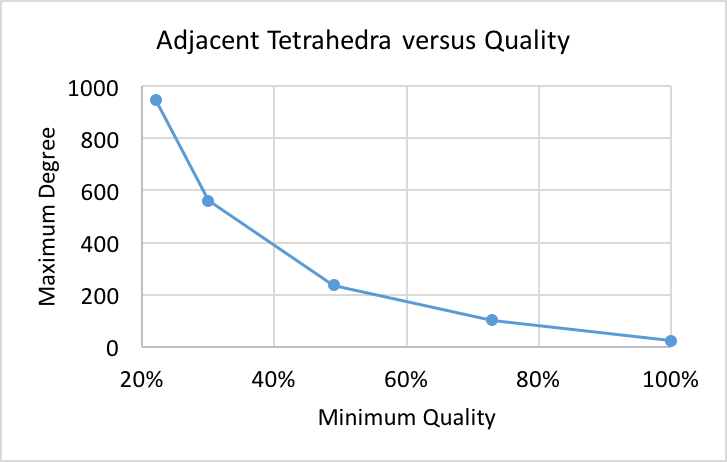
\includegraphics[width=0.6\textwidth]{max_tet_deg.png}
\caption{Maximum vertex-tetrahedron degree given a minimum tetrahedron mean ratio}
\label{fig:max_tet_deg}
\end{center}
\end{figure}

A similar yet much simpler analysis, applied to triangles
from the origin to the edge of a unit circle, results in the
plot given by Figure \ref{fig:max_tri_deg}.

\begin{figure}
\begin{center}
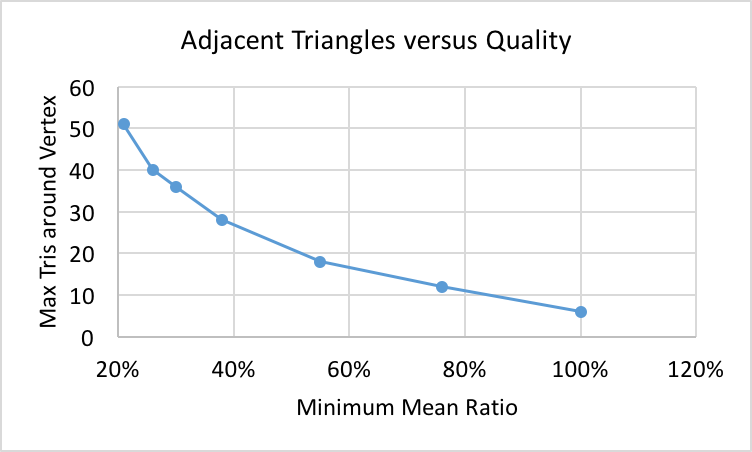
\includegraphics[width=0.6\textwidth]{max_tri_deg.png}
\caption{Maximum vertex-triangle degree given a minimum triangle mean ratio}
\label{fig:max_tri_deg}
\end{center}
\end{figure}
